\section{Protocolli}

Analizzando le tempistiche di detection per i tre protocolli principali utilizzati in questi esperimenti (ICMP, TCP ed UDP) si nota innanzitutto come i tempi di rilevamento per attacchi basati su ICMP (ad es. ping) sia pressoché nulla, rendendo inefficace un qualsiasi tipo di attacco. Per quanto riguarda invece TCP e UDP notiamo un netto distacco, a favore di TCP, secondo i tempi di detection: è possibile, dato che UDP è un protocollo non affidabile che punta tutto sulla velocità d'invio, che gli attacchi basati su UDP siano progettati in modo da agire velocemente, velocizzando quindi anche il processo di rilevazione da parte degli IDS in ascolto, mentre un attacco basato su TCP potrebbe agire più lentamente ed in modo più silenzioso. Un'altra possibile spiegazione è che, dato che il protocollo TCP è affidabile per natura, molte analisi su questi pacchetti vengono già fatte dalla stessa infrastruttura di rete, quindi è possibile che un IDS come Snort decida di dare meno peso (con meno regole o regole meno stringenti) a questo tipo di pacchetti, preferendo invece concentrarsi su pacchetti meno controllati come quelli UDP o ICMP. Osservando invece la durata media degli attacchi raggruppata per protocollo, vediamo come gli attacchi ICMP siano mediamente i più veloci (pensiamo ad attacchi come ping o nmap -I), subito seguiti da attacchi TCP e da attacchi UDP, che evidentemente fanno, in media, più operazioni (o operazioni più complesse) rispetto agli attacchi basati su ICMP o TCP.

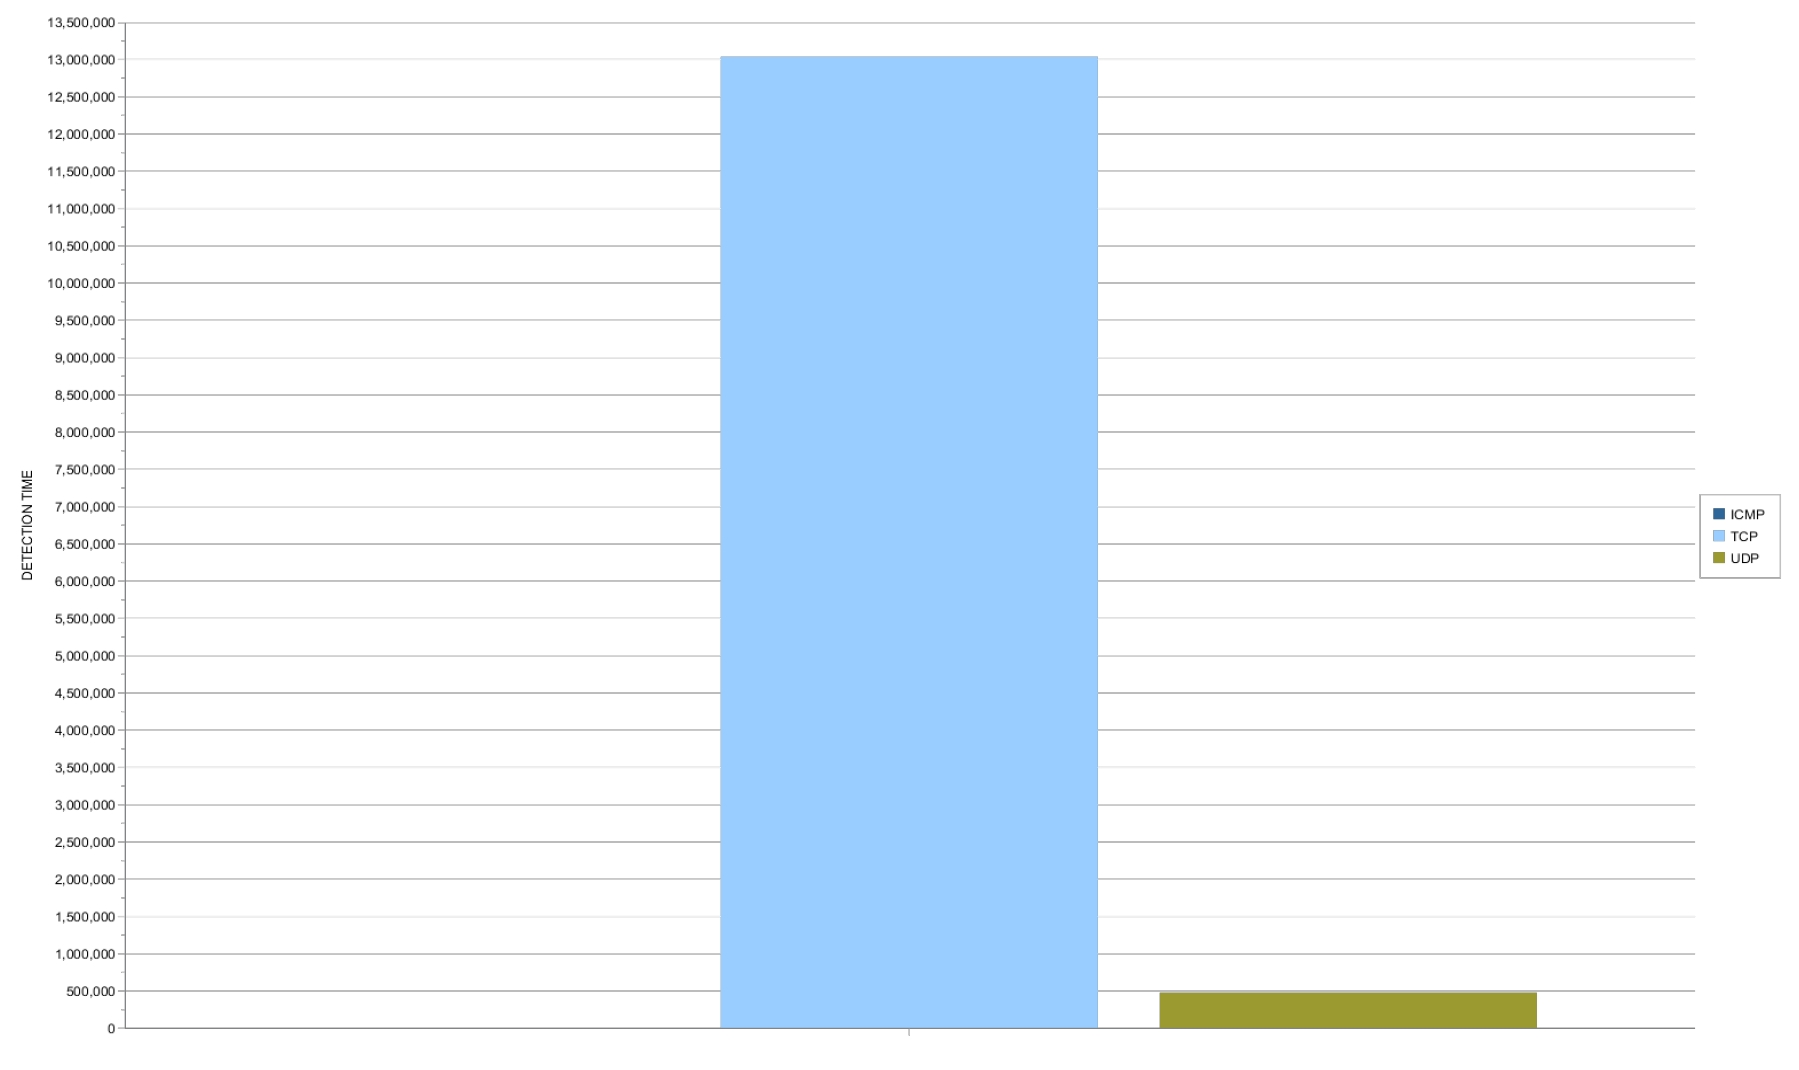
\includegraphics[scale=0.3]{figure/detection_protocol.jpg}\\

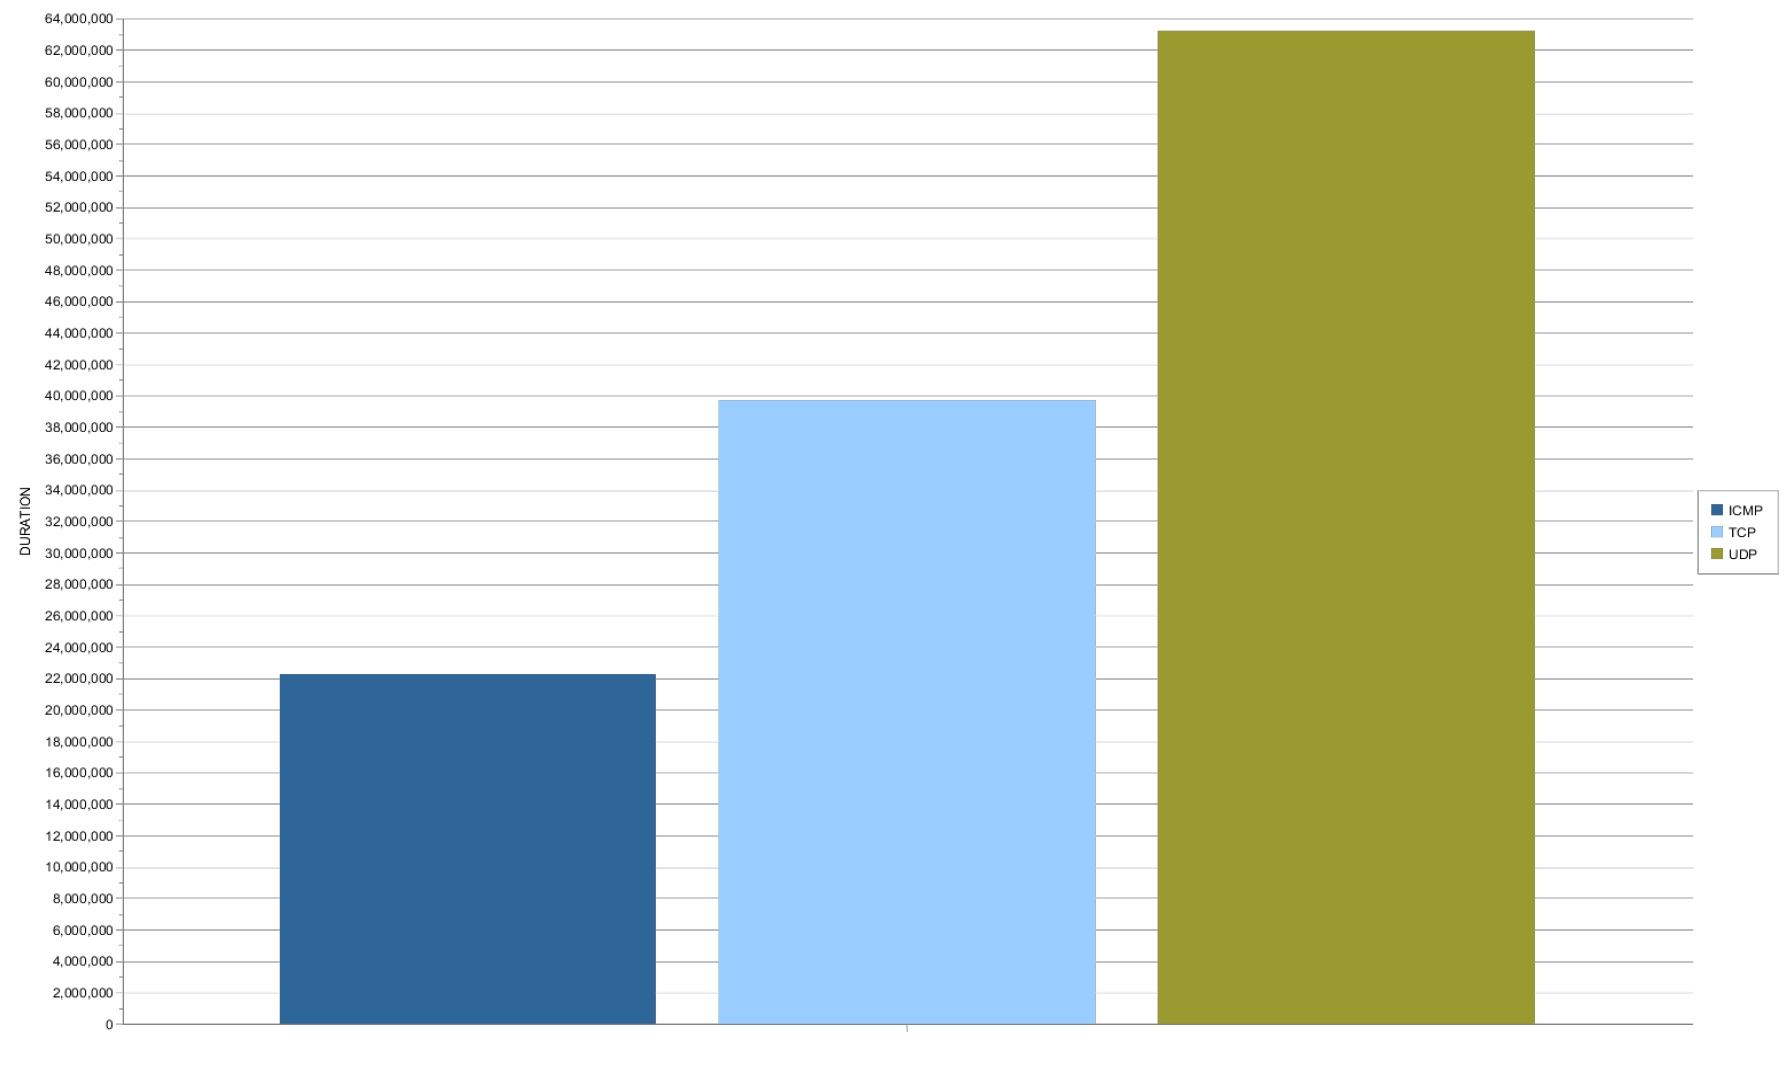
\includegraphics[scale=0.3]{figure/duration_protocol.jpg}\\

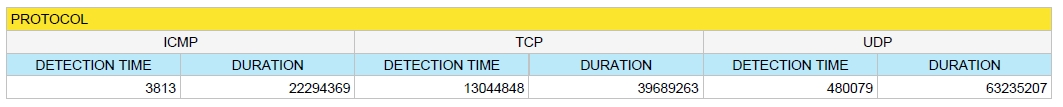
\includegraphics[scale=0.4]{figure/tabella_protocolli.jpg}
